\documentclass{article}
\textheight 22.5truecm \textwidth 14.5truecm
\setlength{\oddsidemargin}{0.35in}\setlength{\evensidemargin}{0.35in}

\usepackage[utf8]{inputenc}
\usepackage[russian]{babel}
\usepackage{graphicx}
\usepackage{amsmath}
\usepackage{breqn}
\usepackage{wrapfig}
\usepackage{float}
\usepackage{multirow}
\usepackage{caption}
\usepackage{subcaption}

\graphicspath{ {./data/images} }
\author{Александр Романов Б01-110}
\date{}
\title{1.3 Изучение рассеяния медленных электронов на атомах (эффект Рамзауэра)}

\begin{document}
\maketitle
\section{Введение}
\subsection{О работе}
Исследуется энергетическая зависимость вероятности рассеяния электронов атомами ксенона, определяются
энергии электронов, при которых наблюдается "просветление" ксенона, и оцениваетчя размер его внешней
электронной оболочки.

\begin{figure}[H]
	\centering
	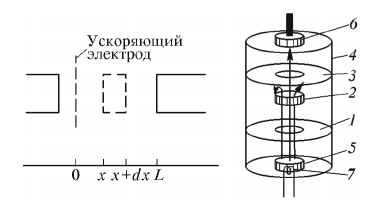
\includegraphics[width=0.6\textwidth]{scheme.png}
	\caption{Схематическое изображение тиратрона (слева) и его конструкция (справа): 
	1, 2, 3 -- сетки; 4 -- внешний металлический циллиндр; 5 -- катод; 6 -- анод;
	7 -- накаливаемая спираль}
\end{figure}

\section{Работа}
Включив все приборы переведём осциллограф в режим внешней развёртки и установим
напряжение накала на уровень \(2.5\;V\). Пронаблюдаем картину вольт-амперной
характеристики эффекта Рамзауэра.

\begin{figure}[H]
	\centering
	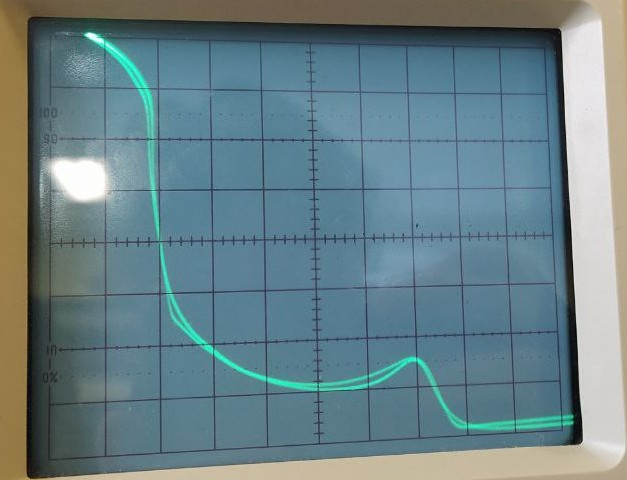
\includegraphics[width=0.6\textwidth]{signal.jpeg}
	\caption{ВАХ эффекта Рамзауэра}
\end{figure}

На изображении отчётливо видны максимумы и минимумы (Отметим что развёртка производится
справа налево).

Проведём расчёт размера электронной оболочки атома инертного газа, заполняющего лампу:

\[ R = \frac{1}{2}\frac{h}{\sqrt{2m(E_1 + U_0)}} = (3.07 \pm 0.05)\;10^{-10}m  \]

Также вычислим глубину потенциальной ямы исходя из данных с осциллографа для двух значений
напряжения накала.
\(V = 2.56\;V\):
\[ U_0 = \frac{4}{5}E_2 - \frac{9}{5}E_1 = 2.00 \pm 0.01 \;V\]
\(V = 2.93\;V\):
\[ U_0 = \frac{4}{5}E_2 - \frac{9}{5}E_1 = 1.56 \pm 0.01\;V\]

Запишем значения напряжения пробоя. \(U_b = 18.6 \pm 0.1\;eV\) для \(U_h = 2.56\;V\) и
\(U_b = 18.6 \pm 0.1\;eV\) для \(U_h = 2.93\;V\). Полученные значения свопадают друг с другом
и лучше всего соотносятся с таковым значением для аргона (\(15.6\;eV\))

Проведём измерения ВАХ тиратрона в статическом режиме установки для двух значений
напряжения накала: \(2.53\;V\) и \(2.97\;V\). Результаты занесём в таблицу и построим графики:

\begin{table}[H]
\centering
\begin{tabular}{|c|c|}
\hline
V, V & I, mA     \\\hline
0.51    & 0.062  \\\hline
1.00    & 0.651  \\\hline
1.15    & 0.994  \\\hline
1.25    & 1.167  \\\hline
1.50    & 1.446  \\\hline
1.60    & 1.570  \\\hline
1.75    & 1.615  \\\hline
1.80    & 1.613  \\\hline
2.00    & 1.498  \\\hline
2.50    & 1.197  \\\hline
3.00    & 0.923  \\\hline
3.50    & 0.762  \\\hline
3.99    & 0.665  \\\hline
4.50    & 0.591  \\\hline
5.00    & 0.550  \\\hline
5.51    & 0.523  \\\hline
6.00    & 0.523  \\\hline
6.50    & 0.541  \\\hline
7.00    & 0.551  \\\hline
7.50    & 0.567  \\\hline
8.00    & 0.586  \\\hline
8.50    & 0.641  \\\hline
9.00    & 0.706  \\\hline
9.51    & 0.814  \\\hline
10.00   & 0.892  \\\hline
10.50   & 0.963  \\\hline
11.00   & 0.109  \\\hline
11.50   & 1.322  \\\hline
11.90   & 1.432  \\\hline
\end{tabular}
	\caption{\(2.53V\)}
\end{table}

\begin{figure}[H]
	\centering
	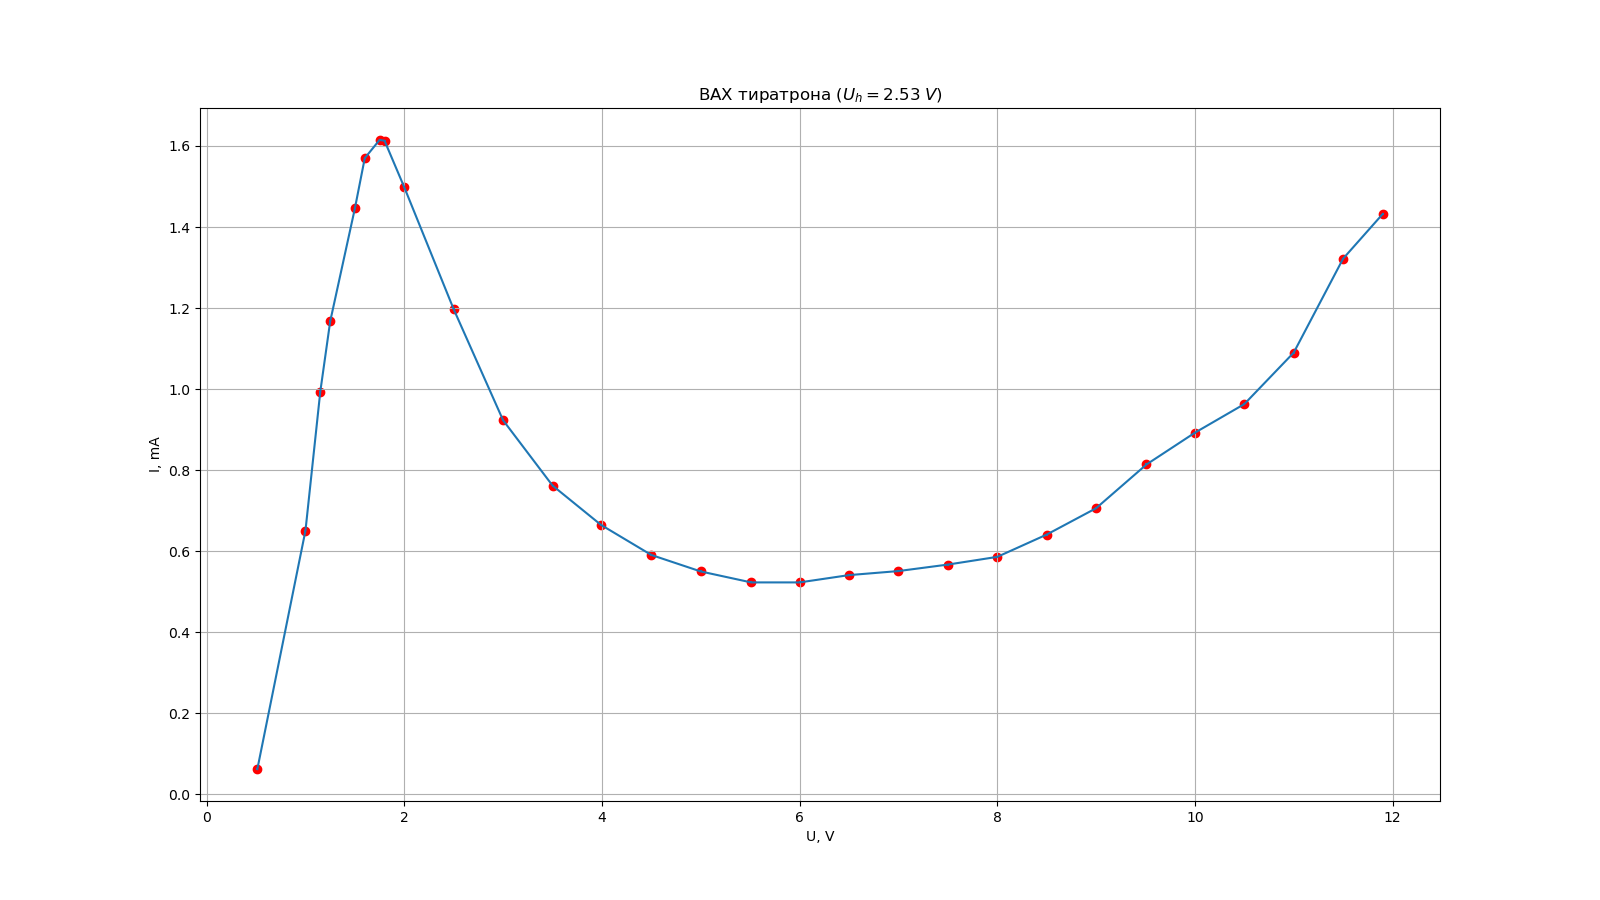
\includegraphics[width=\textwidth]{2.53.png}
	\caption{ВАХ при \(2.53\;V\)}
\end{figure}

\begin{table}[H]
\centering
\begin{tabular}{|c|c|}
\hline
V\_c, V & I, mA  \\\hline
0.13    & 0.006  \\\hline
0.25    & 0.025  \\\hline
0.38    & 0.065  \\\hline
0.50    & 0.134  \\\hline
0.63    & 0.265  \\\hline
0.75    & 0.457  \\\hline
0.88    & 0.696  \\\hline
0.99    & 0.951  \\\hline
1.13    & 1.218  \\\hline
1.25    & 1.417  \\\hline
1.37    & 1.574  \\\hline
1.50    & 1.672  \\\hline
1.63    & 1.726  \\\hline
1.75    & 1.740  \\\hline
1.87    & 1.727  \\\hline
2.00    & 1.694  \\\hline
2.12    & 1.650  \\\hline
2.22    & 1.609  \\\hline
2.38    & 1.543  \\\hline
2.40    & 1.531  \\\hline
2.60    & 1.452  \\\hline
2.80    & 1.380  \\\hline
3.00    & 1.322  \\\hline
3.21    & 1.274  \\\hline
3.40    & 1.239  \\\hline
3.59    & 1.210  \\\hline
3.80    & 1.187  \\\hline
4.00    & 1.168  \\\hline
4.20    & 1.150  \\\hline
4.51    & 1.133  \\\hline
5.00    & 1.134  \\\hline
5.50    & 1.137  \\\hline
6.00    & 1.180  \\\hline
6.50    & 1.243  \\\hline
6.99    & 1.312  \\\hline
7.50    & 1.403  \\\hline
8.02    & 1.520  \\\hline
8.51    & 1.650  \\\hline
9.00    & 1.813  \\\hline
9.50    & 2.080  \\\hline
10.00   & 2.300  \\\hline
10.60   & 2.600  \\\hline
11.07   & 2.900  \\\hline
11.50   & 3.300  \\\hline
11.50   & 3.300  \\\hline
\end{tabular}
\caption{\(2.97\;V\)}
\end{table}

\begin{figure}[H]
	\centering
	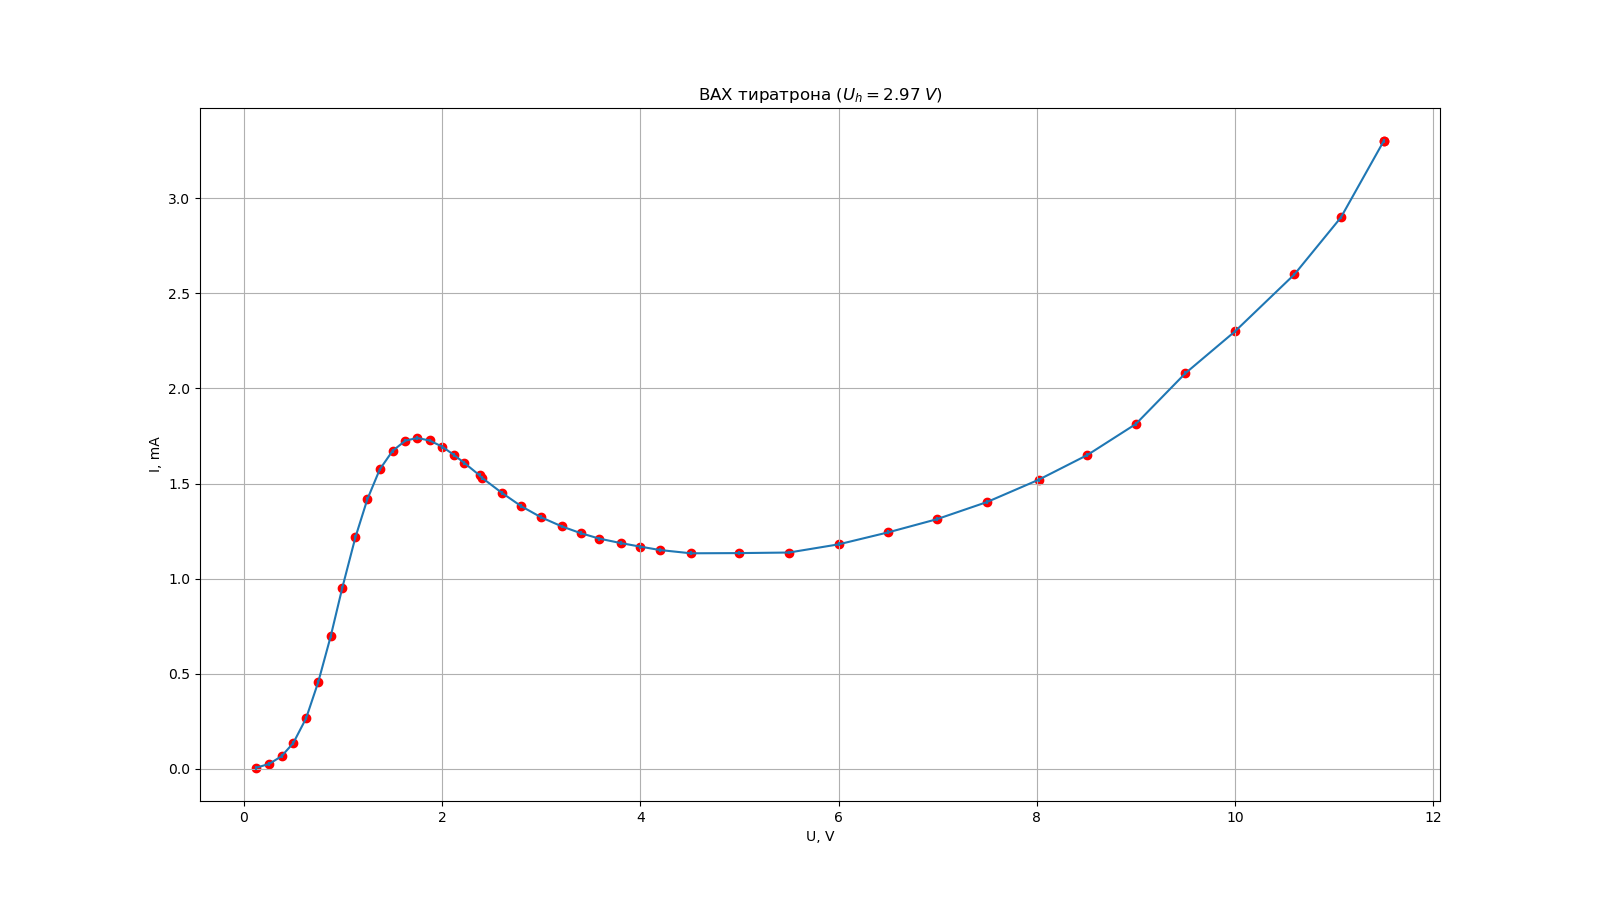
\includegraphics[width=\textwidth]{2.97.png}
	\caption{ВАХ при \(2.97\;V\)}
\end{figure}

В приведённых выше данных везде погрешность составляет \(\Delta V = 0.01\;V\) и
\(\Delta I = 0.001\;mA\).
Оценим при каких напряжениях должны появиться максимумы в коэффициенте прохождения электронов.
Используем формулу:
\[ k_2R = \sqrt{\frac{2m(E_n + U_0)}{\hbar^2}}R = n\pi\]
\[ n = \sqrt{\frac{E_n + U_0}{E_1 + U_0}} \]
\[ E_n = n^2\left(E_1 + U_0\right) - U_0 \]
\[ E_2 = 4\left(E_1 + U_0\right) - U_0 = (14.0 \pm 0.1) eV\]
\[ E_3 = 4\left(E_1 + U_0\right) - U_0 = (34.0 \pm 0.1) eV\]

Вычислим зависимость вероятности рассеяния электрона от его энергии из соотношения (Возьмём 
\(C = 1\)):
\[ \omega\left(V\right) = -\frac{1}{C}\ln{I(V)/I_0} \]

\begin{figure}[H]
	\centering
	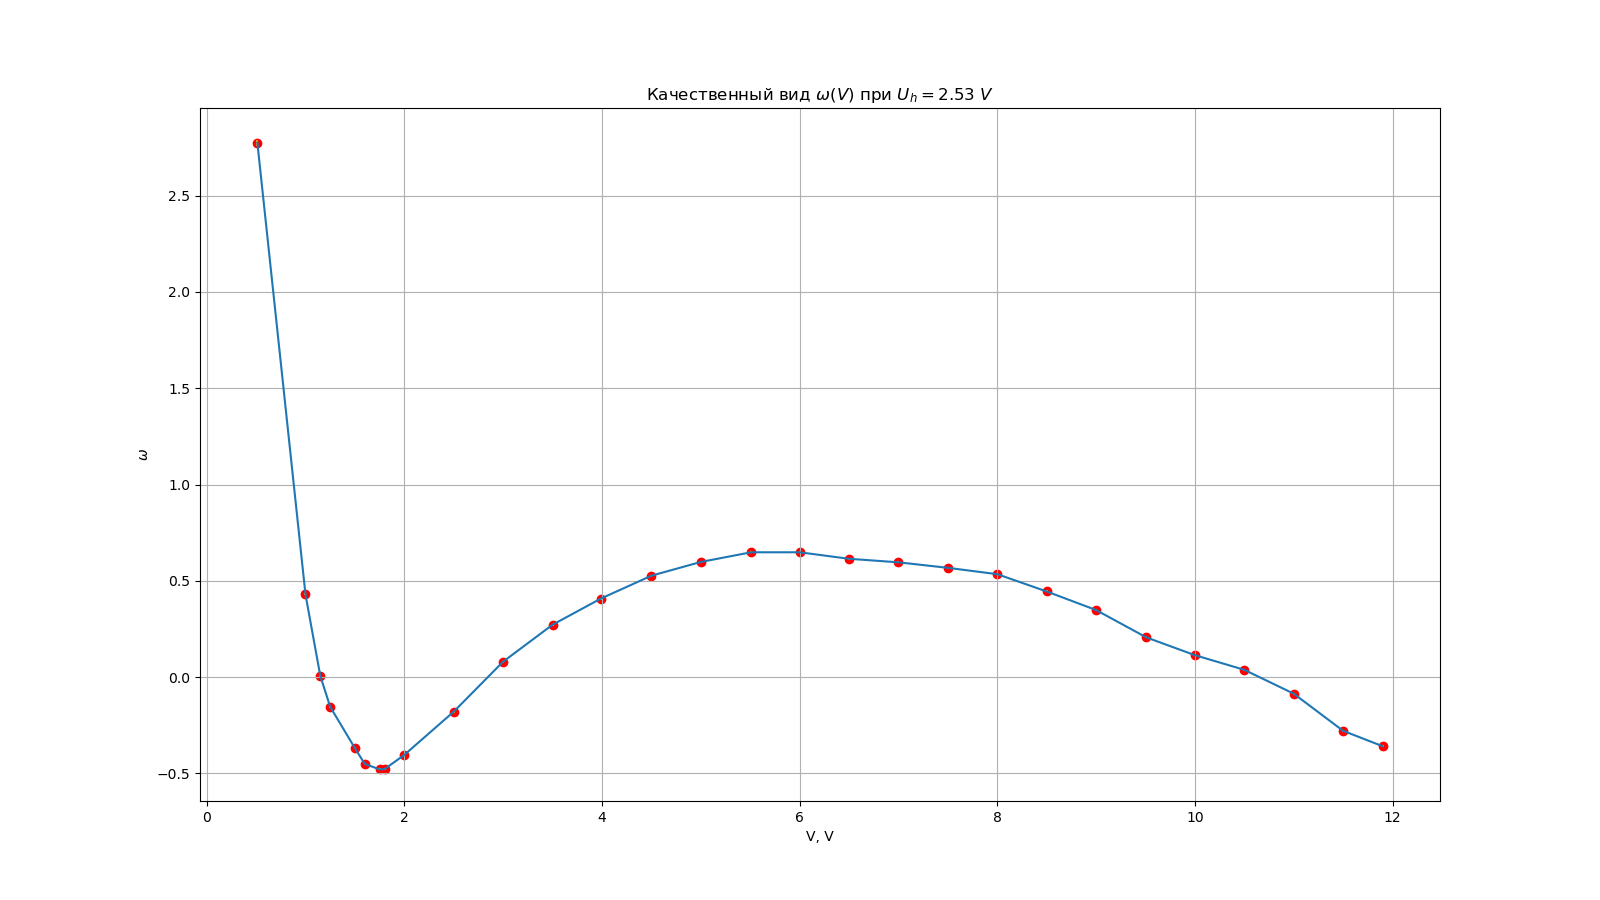
\includegraphics[width=\textwidth]{omega2.53.png}
	\caption{\(\omega\left(V\right)\) при \(U_h = 2.53\;V\)}
\end{figure}
\begin{figure}[H]
	\centering
	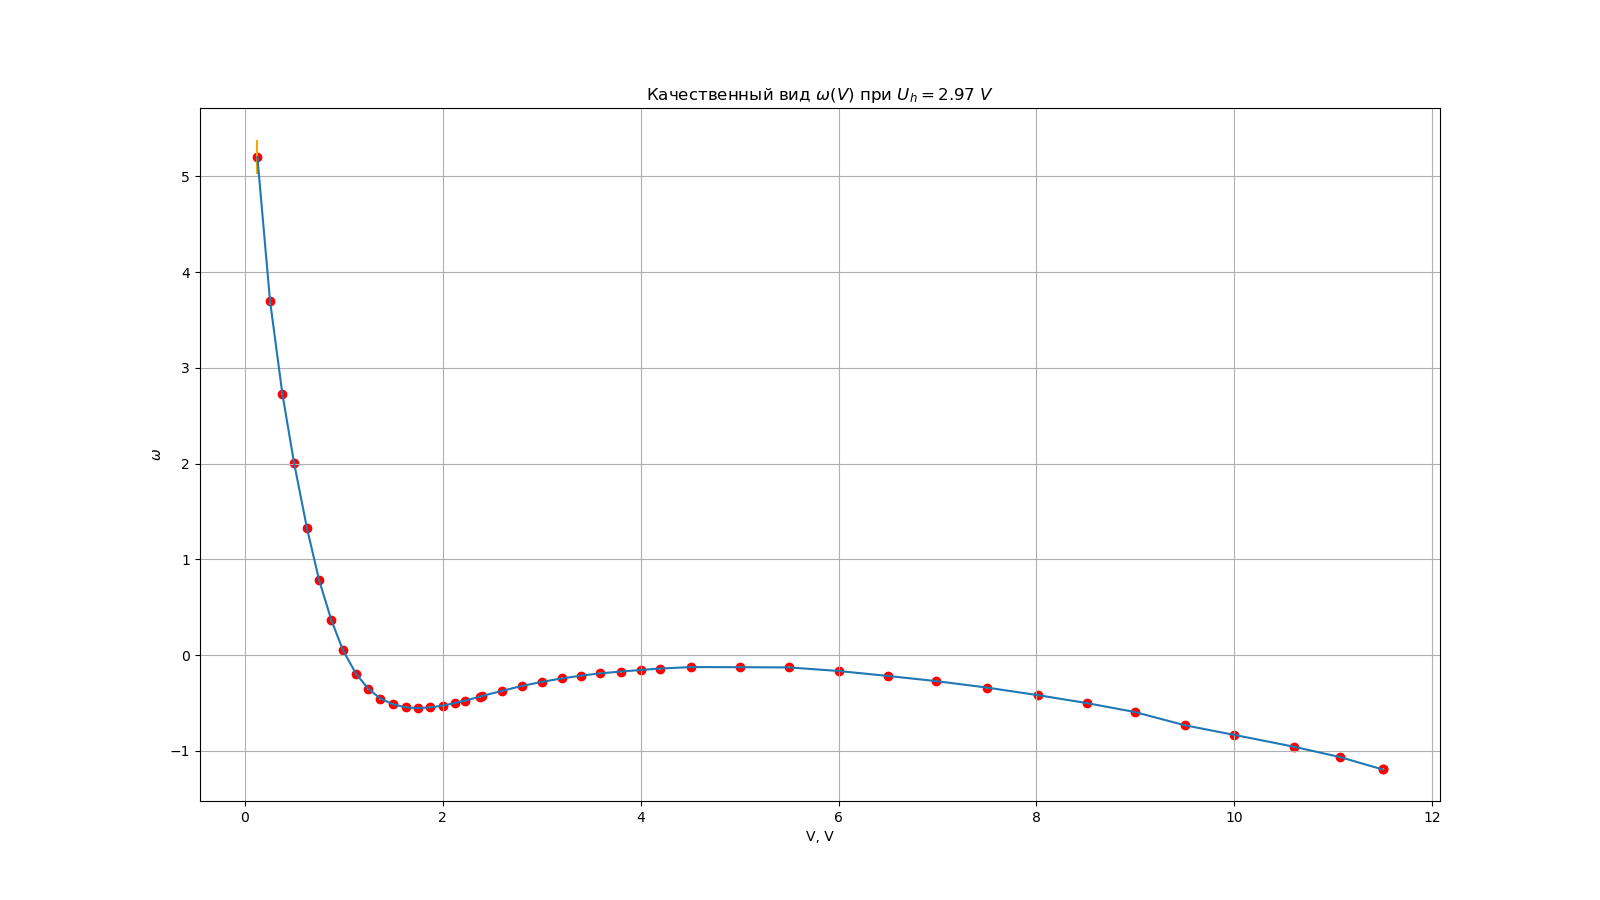
\includegraphics[width=\textwidth]{omega2.97.png}
	\caption{\(\omega\left(V\right)\) при \(U_h = 2.97\;V\)}
\end{figure}

\section{Выводы}
В ходе выполнения работы:
\begin{enumerate}
	\item Был измерен размер внешней электронной оболочки ксенона 
(\((3.07 \pm 0.05)\;10^{-10}m\)). Полученной значение выглядит крайне правдоподобным.
	\item Бфли оценены значения максимумов просветления ксенона:
		\[E_2 = (14.0 \pm 0.1)\;eV\]
		\[E_3 = (34.0 \pm 0.1)\;eV\]
	\item Была измерена зависимость вероятности рассеяния электрона от его энергии.
\end{enumerate}

\end{document}
